\subsection{Decider and DeciderToPhy interface}
\label{decider}

The main task of the Decider is to decide which packets should be handed up to
the MAC layer. To achieve this the \h{\bp} hands every receiving AirFrame
several times to the ``processSignal()``- function of the Decider.

\label{ProcessSignal}
The most common case how a Decider would process AirFrames would be the
following:

\begin{enumerate}
 \item If the Decider gets an AirFrame for the first time, it determines the
time point it can decide if the packet is noise or not and returns this time
point to the \h{\bp}. The time point could be the preamble length, for example.

 \item The next time the Decider gets the packet it would internally decide if
the packet has to be considered noise or not. If the decision is noise the
packet isn't interesting anymore for the Decider. If the packet is classified
as a signal the Decider would return the end of the signal to the \h{\bp}.

 \item When the receiving of the AirFrame is over and the AirFrame wasn't
classified as noise, the Decider would decide if the packet was received
correctly. If the result is positive the Decider has to tell the \h{\bp} to
send the AirFrame together with the DeciderResult to the \h{\bm}.
\end{enumerate}

A second task of the decider is to decide if the channel is busy or idle at a
specific point in time or during a given interval.\\

Since the Decider is responsible to decide if an AirFrame should be
decapsulated and handed up to the MAC layer the Decider needs an interface to
the \h{\bp}.\\

Over the interface the Decider can do the following things:

\begin{itemize}
 \item get the current simulation time
 \item get the list of AirFrames which intersect which a specific interval (to
calculate SNR)
 \item tell the \h{\bp} to hand an AirFrame up to the MAC layer
 \item tell the \h{\bp} to send a control message to the MAC layer
\end{itemize}

Due to the last point the Decider is able to answer a ChannelSenseRequest of the
MAC layer.\\

A Decider that gives a more detailed DeciderResult (e.g. bitwise
errors\req{defdeciderBitwise}) must be subclassed and implemented by the user.

\begin{figure}[H]
 \centering
 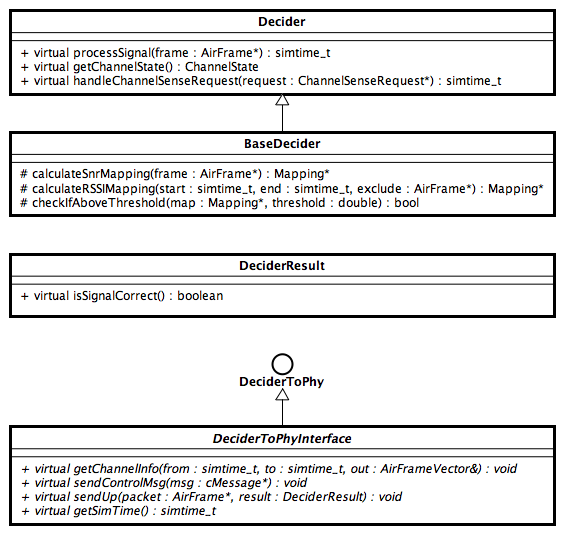
\includegraphics[width = \textwidth]{modelling/DeciderModule_members.png}
 \caption{Decider interface}
 \label{fig: Decider interface}
\end{figure}

\newpage

\subsection{The one-dimensional Signal and AirFrame}
\label{AirFrame and Signal}

AirFrame and Signal both hold information about the packet to send. While the
AirFrame is responsible for the OMNeT related data which is necessary to send
OMNeT messages, the Signal holds the data which is necessary for the simulation
of the transmission process.\\

Here we focus on the basic, one-dimensional (time) Signal that stores entries
for TX Power and attenuation over time\footnote{The time stamps are values
relative to starting time point}. There are fix entries for header and
payload bitrate. These assumptions are considered to cover most cases.
It is possible to obtain a time iterator for this Signal to have access to
entries at specific time points.

Further Signal stores the Move (move pattern of the sending host), the packets
header length, the start time and length of the Signal.\\

\emph{Note: The multi-dimensional Signal is an instance of the same class but
has more functionality. It is described in detail in a separate section.}\\

To be able to control the sending process\req{defsendControl} of an AirFrame
every AirFrame has a unique id and a specific type which specifies if this is a
normal AirFrame or a control-AirFrame. Further it holds an instance of Signal
which represents the physical signal.


\begin{figure}[H]
 \centering
 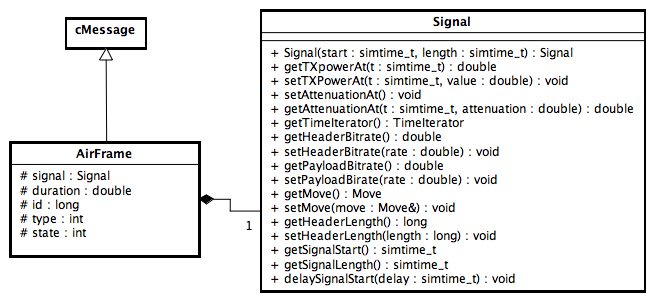
\includegraphics[width = \textwidth]{modelling/AirFrame_members.png}
 \caption{member arrangement in AirFrame and Signal}
 \label{fig:memberAirFrame}
\end{figure}
\newpage

\subsection{receiving a MacPkt}

On reception of a MacPkt from the MAC layer, \h{\bp} checks if:
\begin{enumerate}
	\item the radio is in TX state\req{defsendPreqMode},
	\item it is not already sending a packet\req{defsendPreqSending} 
\end{enumerate} 

If one of these conditions is not fulfilled it will throw an error.\\

The MacToPhyControlInfo object attached to the MacPkt contains the information
needed by \h{\bp} when constructing the AirFrame to send to the channel.
Right now it only contains the Signal initialized by the \h{\bm}.

See \ref{SignalCreation} for how the Signal is created by the \h{\bm}.

\begin{figure}[H]
 \centering
 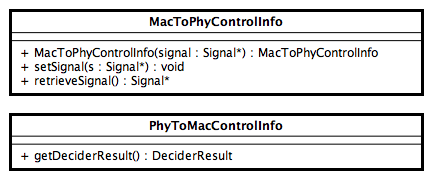
\includegraphics[width = \textwidth]{modelling/MacToPhyCtrlInfo_members.png}
 \caption{MacToPhyControlInfo interface}
 \label{fig: MacToPhyCtrlInfo interface}
\end{figure}


\h{\bp} adds further information to the Signal and is responsible for creating
and initializing the AirFrame and attaching the Signal to it.
For detailed arrangement of information in Signal and AirFrame see \ref{AirFrame
and Signal}.
When the AirFrame is complete and sent, \h{\bp} schedules a TX\_OVER message to
the \h{\bm} (via control-message).

\begin{figure}[H]
 \centering
 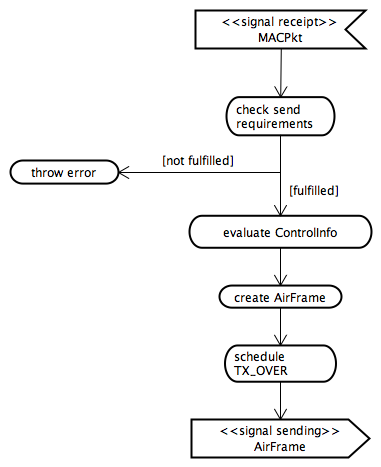
\includegraphics[width = 0.8\textwidth]{modelling/onMACPkt.png}
 \caption{sending process}
 \label{fig: sending process}
\end{figure}
\newpage



\subsection{Receiving and processing an AirFrame}

On arrival of an AirFrame \h{\bp}:
\begin{enumerate}
	
	\item applies AnalogueModels to the corresponding
Signal\req{defrcvSimAttenuation},
	\item receives the AirFrame\req{defrcvSimDuration}.
\end{enumerate}

\begin{figure}[H]
 \centering
 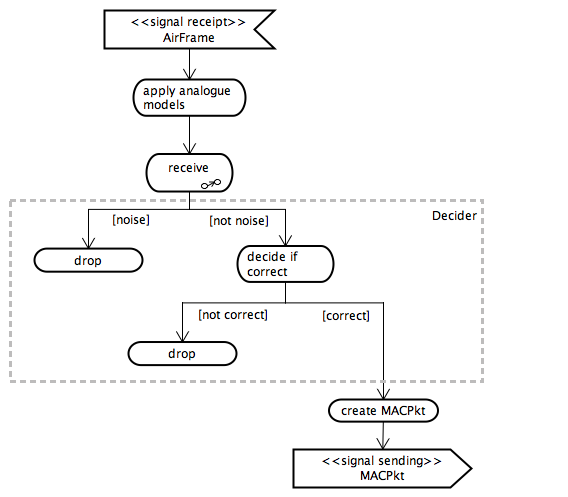
\includegraphics[width = \textwidth]{modelling/onAirFrame.png}
 \caption{receiving process}
 \label{fig: receiving process}
\end{figure}


The receiving process works as follows: In general, time intervals during
reception are simulated by scheduling the AirFrame accordingly.\\

\textbf{stage 0:}\\
An optional propagation delay is simulated by updating the starting time of the
Signal\req{defrcvSimDelay} according to the delay and scheduling the AirFrame to
the reception start point.\\

\textbf{stage 1:}\\
On reception start the Signal is given to the Decider for processing. The
Decider returns a time point it wants to process the Signal again.
This time point has to be before the end of the Signal otherwise an error
is thrown. \\

\textbf{stage 2:}\\
The AirFrame is scheduled arbitrary times for the Decider processing method
until it either returns a negative time point or the time point of the end of
the
Signal. In both cases the state is increased by one before the AirFrame is
scheduled to its end. See \ref{ProcessSignal} for more details on the Deciders
Signal processing. \\

\textbf{stage 3:}\\
Finally reception is over and the AirFrame is completely received in reality.

\emph{Note: The Decider process is responsible for telling the \h{\bp} to send
a MacPkt to the \h{\bm}.}

\begin{figure}[H]
 \centering
 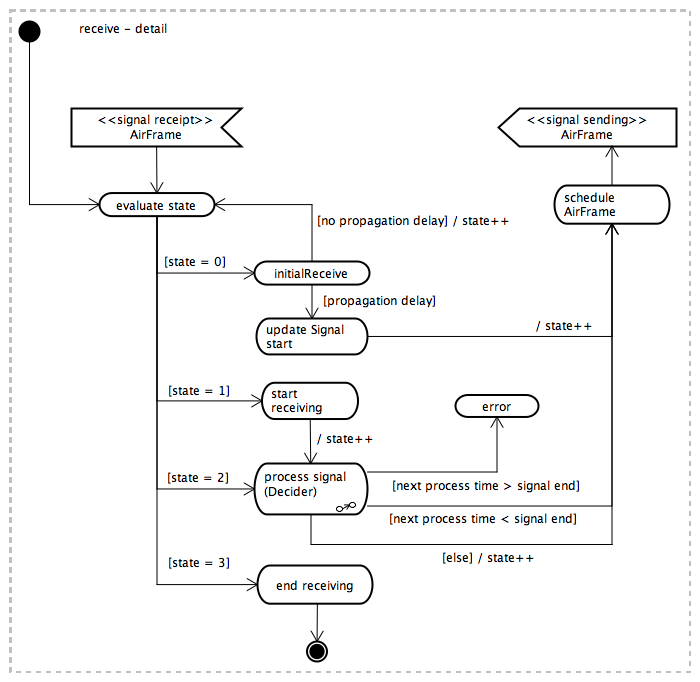
\includegraphics[width = \textwidth]{modelling/receive_detail.png}
 \caption{receive detail}
 \label{fig: receive detail}
\end{figure}


% The receiving process is modelled internally by a state machine that schedules
%the AirFrame that is received (since we have a pointer to it from the
%beginning) everytime a delay/time interval shall be simulated. That saves us
%the creation of additional self-messages.




%When the preamble of a packet is completely received, \h{\bp} constructs a
%SNInfo for the preamble, applies the AnalogueModels to it and passes it to the
%Decider to find out whether this packet is considered noise.

%\begin{figure}[H]
% \centering
% \includegraphics[width = 0.2\textwidth]{modelling/end_preamble_detail.png}
% \caption{end preamble detail}
% \label{fig: end preamble detail}
%\end{figure}

%In case a received packet is not \textit{noise} it is processed, i.e. \h{\bp}
%creates the corresponding SNInfo for the packet, applies AnalogueModels to it
%and passes the result to the Decider to check whether the packet was received
%correctly. If so, a MacPkt is created and handed up to
%Phy-Layer\req{defrcvPassToMAC}.


\subsection{the .ned-file}

The .ned-file of the \h{\bp} has the following parameters:

\begin{itemize}
\item usePropagationDelay as \textit{boolean}\req{defconfDelay}
\item analogueModels as
\textit{XML}\req{defconfAnalogue}\req{defconfAnalogueParam}
\item decider as \textit{XML}\req{defconfDecider}\req{defconfDeciderParam}
\item thermalNoise as \textit{numeric const}\req{defconfNoise}
\item sensitivity as \textit{numeric const}\req{defconfSens}
\item maximal TX power as \textit{numeric const}\req{defconfMaxTXPower}
\item switchTimeRX as \textit{numeric const}\req{defconfSwitchingTimes}
\item switchTimeTX as \textit{numeric const}\req{defconfSwitchingTimes}
\item switchTimeSleep as as \textit{numeric const}\req{defconfSwitchingTimes}
\end{itemize}

The parameters "analogueModels" and "decider" store which AnalogueModels and
which Decider are to be used, together with their parameters in XML format. The
exact format still has to be declared!

%\subsection{provide status information to MAC}

%Passively provided information\req{defprovpassive}: \h{\bm} is equipped with a
%reference to \h{\bp} in order to obtain information
%about channelstate\req{defchannelstate} and current radio
%state\req{defcurrentmode}
%by
%simple method calls. \\
%Actively provided information\req{defprovactive}: A cMessage of the kind
%TX\_OVER
%is sent to MAC layer when a sending transmission is over\req{deftxover},
%\saf{sending process}.



%\subsection{send packets}

%Since \h{\bm} has a reference to \h{\bp} it can obtain information about the
%state the radio is is currently in\req{defsendPreqMode}, it is not already
%sending
%to the channel on its own\req{defsendPreqSending} and the channel is
%idle\req{defsendPreqIdle} via method calls, \saf{BasePhyLayer interface}.

%The class MacToPhyControlInfo is designed as the container for control
%info\req{defpacketFromMac} the MAC layer
%wants to attach to the packet given down to Phy-Layer for sending.
%The packet itself is handed down as a MacPkt via OMNeT-channel. 